\documentclass{article}
\usepackage{graphicx} % Required for inserting images
\usepackage{fancyhdr}
\usepackage{dirtree}


\title{MINI GAME HUB}
\author{Machupalli Bhavya \\ Yanala Subha Srivalli Athreyi }
\date{Spring 2025-26}

\pagestyle{fancy}
\lhead{Mini Game Hub}
\rhead{CS-108 25-26}

\begin{document}

\maketitle

\tableofcontents
\newpage
\section{Introduction}
The aim of this project is to build a two player game hub that integrates bash for authentication , python for gameplay and pygame for GUI. 

After signing in, two players choose a game from the menu, compete using an interactive graphical interface, and their performance is automatically recorded on a long-term leaderboard.

\section{Modules Used}
\begin{itemize}
    \item \textbf{pygame-ce:} It is used in this project to simplify the development process by handling graphical rendering, user input, and core game operations, allowing the focus to remain on designing and managing the interactive gameplay experience\cite{pygame}.
    \item \textbf{numpy:} It is used to efficiently handle the array based operations making tasks like managing grid data, calculations, and game logic faster and more organized.\cite{numpy}
    \item \textbf{matplotlib:} Matplotlib is used in this project to turn data like scores and performance into clear visual graphs, making it easier analyze the results.\cite{matplotlib}
    \item \textbf{datetime:} It is used to get the date and time at certain point i,e; when the game history is stored.
    \item \textbf{sys:} sys is used in the project to handle basic things like closing the program properly and dealing with any inputs given when it starts, so everything runs smoothly.
    \item \textbf{subprocess:} It is used to run different scripts within the main program , helping different parts to work together smoothly.
    
\end{itemize}

\section{Directory Structure}
The project directory is as follows:
\dirtree{%
        .1 \hspace{1.5pt}..
        .2 main.sh.
        .2 game.py.
        .2 games.
        .3 connect4.py.
        .3 othello.py.
        .3 tictactoe.py.
        .3 X.png.
        .3 O.png.
        .2 leaderboard.sh.
        .2 users.tsv.
        .2 history.csv.
        .2 report.
}

\begin{itemize}
    \item \textbf{main.sh:} Bash script for user authentication.
    \item \textbf{game.py:} game.py receives the two authenticated usernames and manages the full Python-side flow: the game menu, gameplay, post-game recording, and analytics.
    \item \textbf{users.tsv:}File that stores the information of registered user i.e; Username and Hashed password
    \item \textbf{games:}A folder containing the game classes for each of \textit{TicTacToe, Othello, Connect4} and images for tictactoe.
    \item \textbf{history.csv:} File that stores the data of winner, loser, data and time played and the game played.
    \item \textbf{leaderboard.sh:}Bash script to print the leaderboard on terminal.
    
\end{itemize}

\section{How to run the program?}
\subsection{Pre-requisites}
Make sure that python 3.10 is already installed in your system\cite{python}.\\
Install the required libraries  using:\\ \\
\texttt{pip install pygame-ce matplotlib numpy}\\
\\
Open the project folder in your terminal and 
run the main file using:\\ \\
\texttt{bash main.sh}\\ \\
It asks to login /register if required.
After the authentication bash runs :\\ \\
\texttt{python3 game.py username1 username2}

\subsection{Game Navigation}
Once both the players are authenticated , the main game interface is launched.\\

After logging in, a graphical menu is displayed using Pygame, showing different game options like Tic Tac Toe, Othello, and Connect4. Players can choose a game by simply clicking on the option they want on the screen.
\newpage
 \begin{figure}[h!]
        \centering
        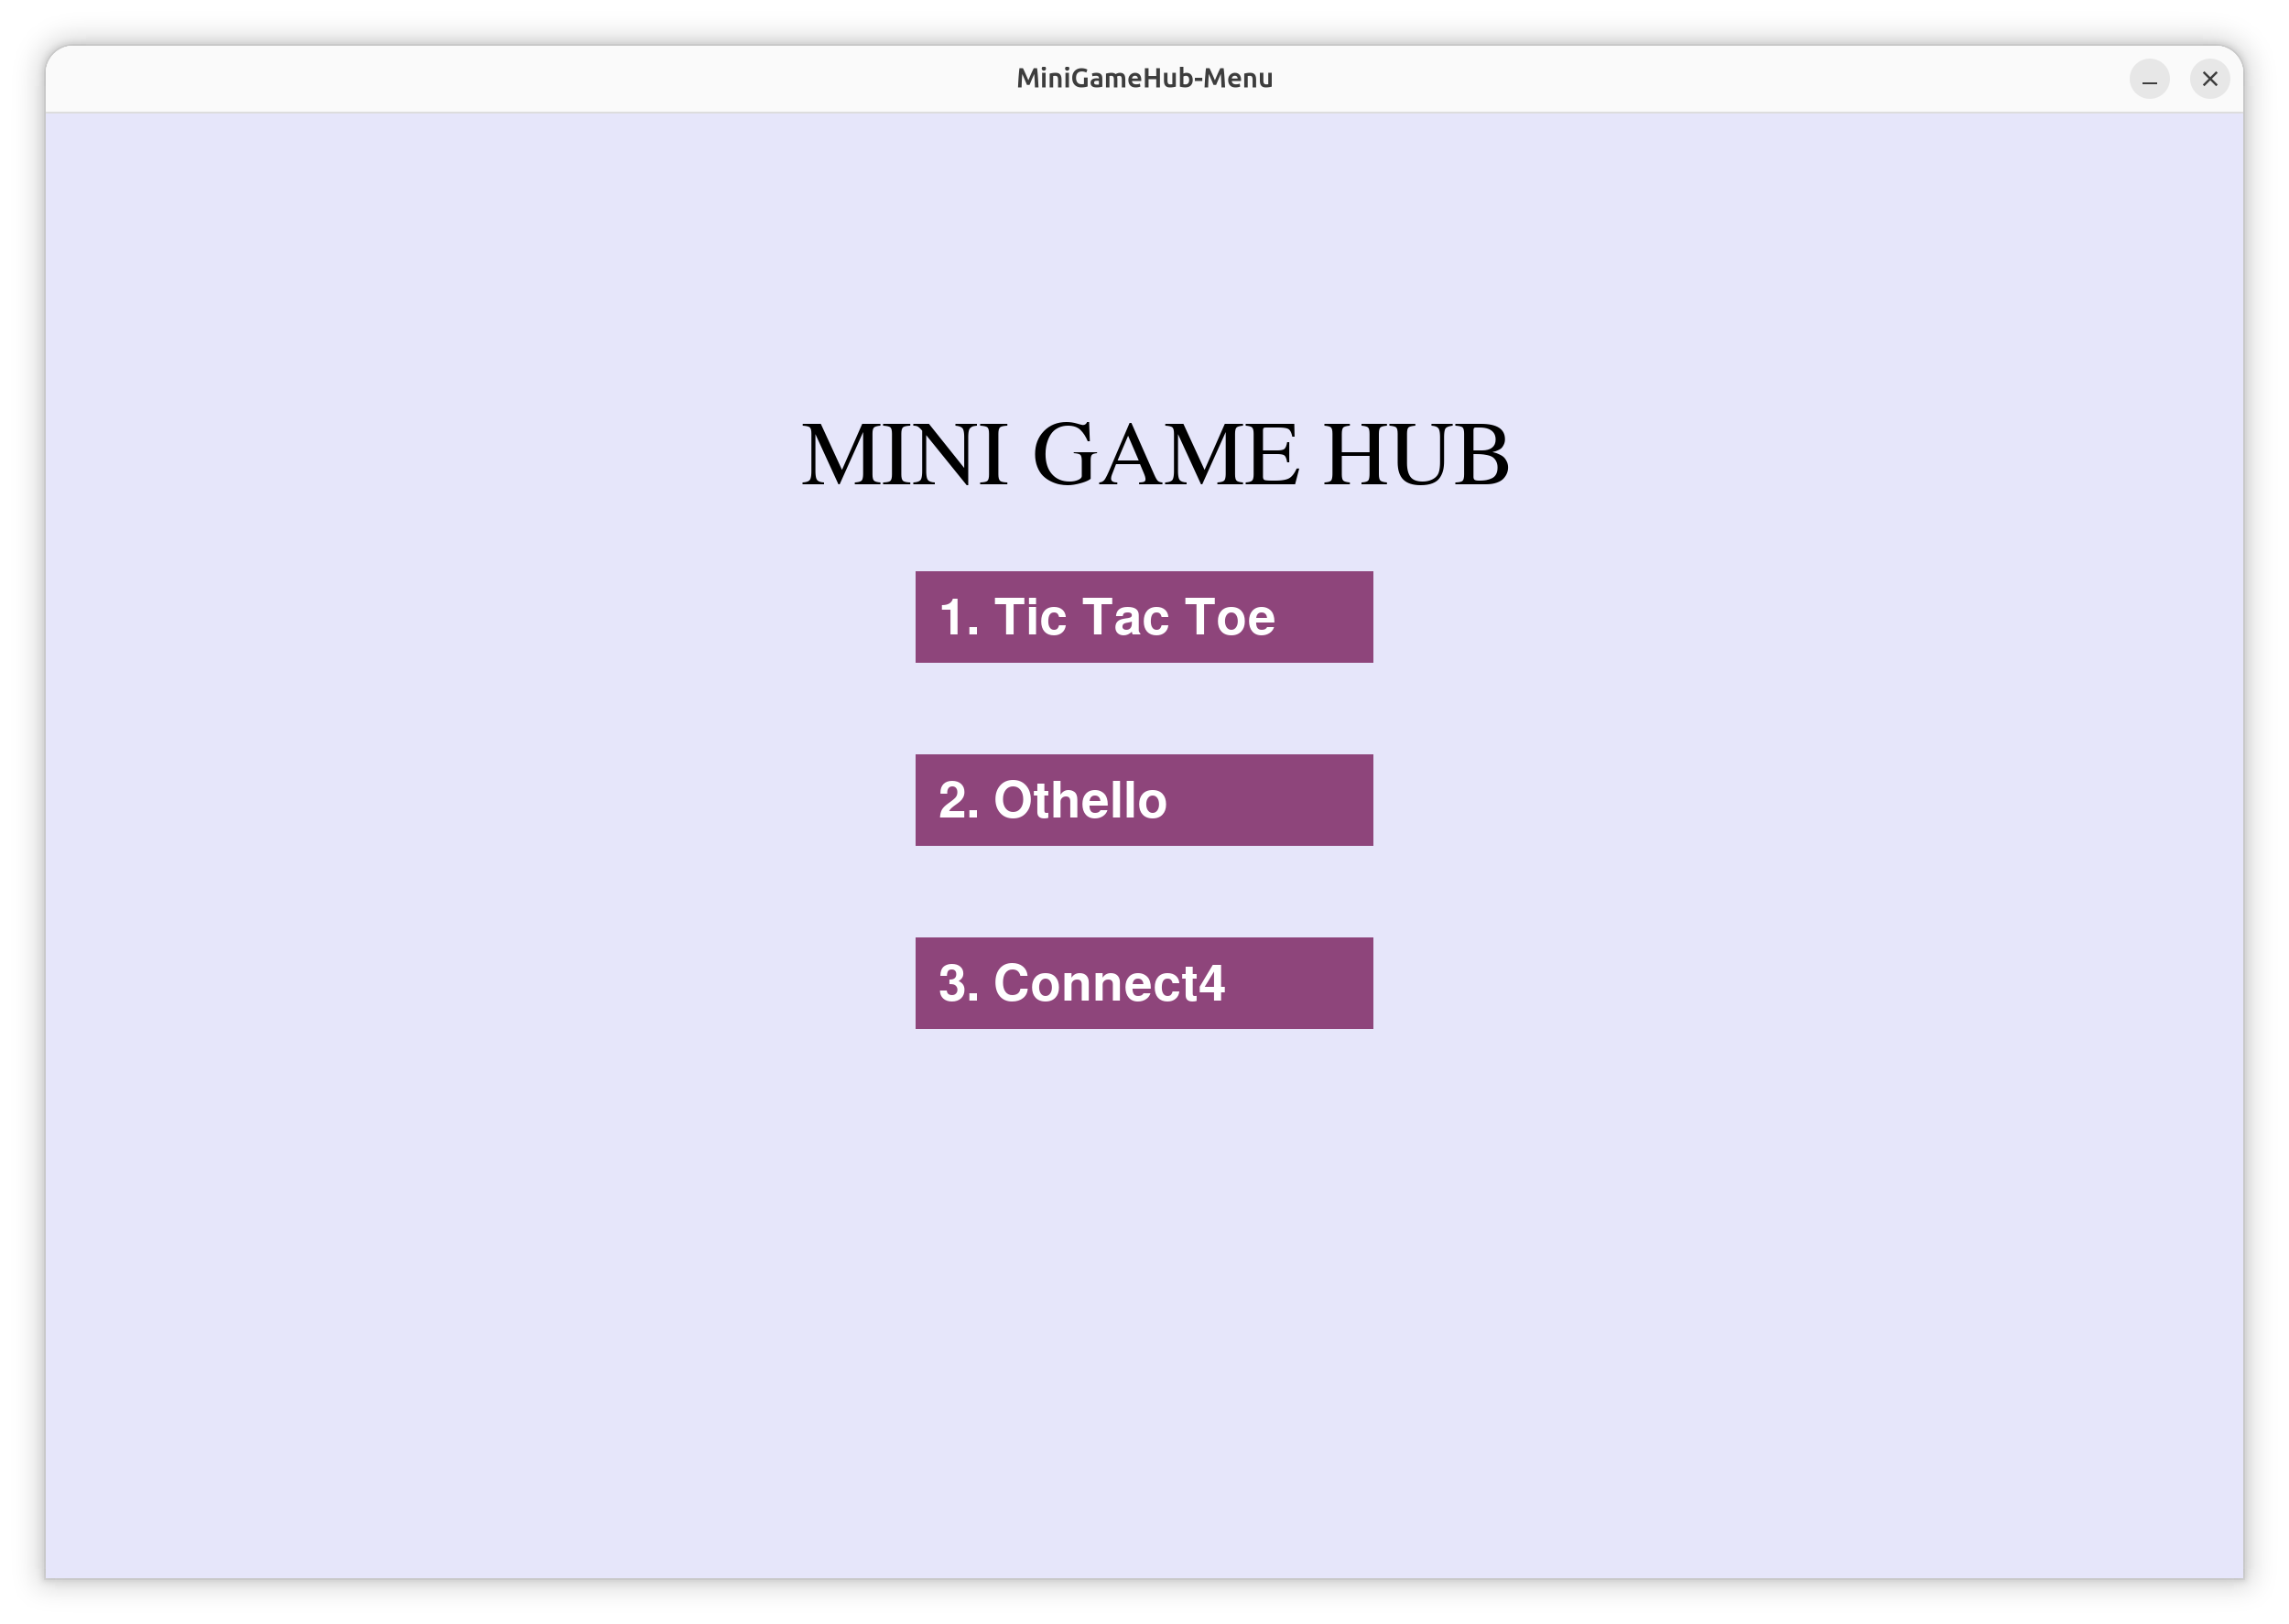
\includegraphics[width=0.8\textwidth]{Images/Game menu.png}
        \caption{Menu Screen}\label{fig:Menu Screen}
    \end{figure}
Once you chose a game, it opens up with its own interface and you can start playing right away. When the game finishes, the result is saved automatically, and the leaderboard is shown so you can see how players are performing, with options to sort it by things like player name, No. of Wins, No. of losses, and by win-loss ratio. \\
\textbf{Note:} Players can chose the sort factor on GUI window that launches after the game has ended and view the leaderboard on the terminal.

 \begin{figure}[h!]
        \centering
        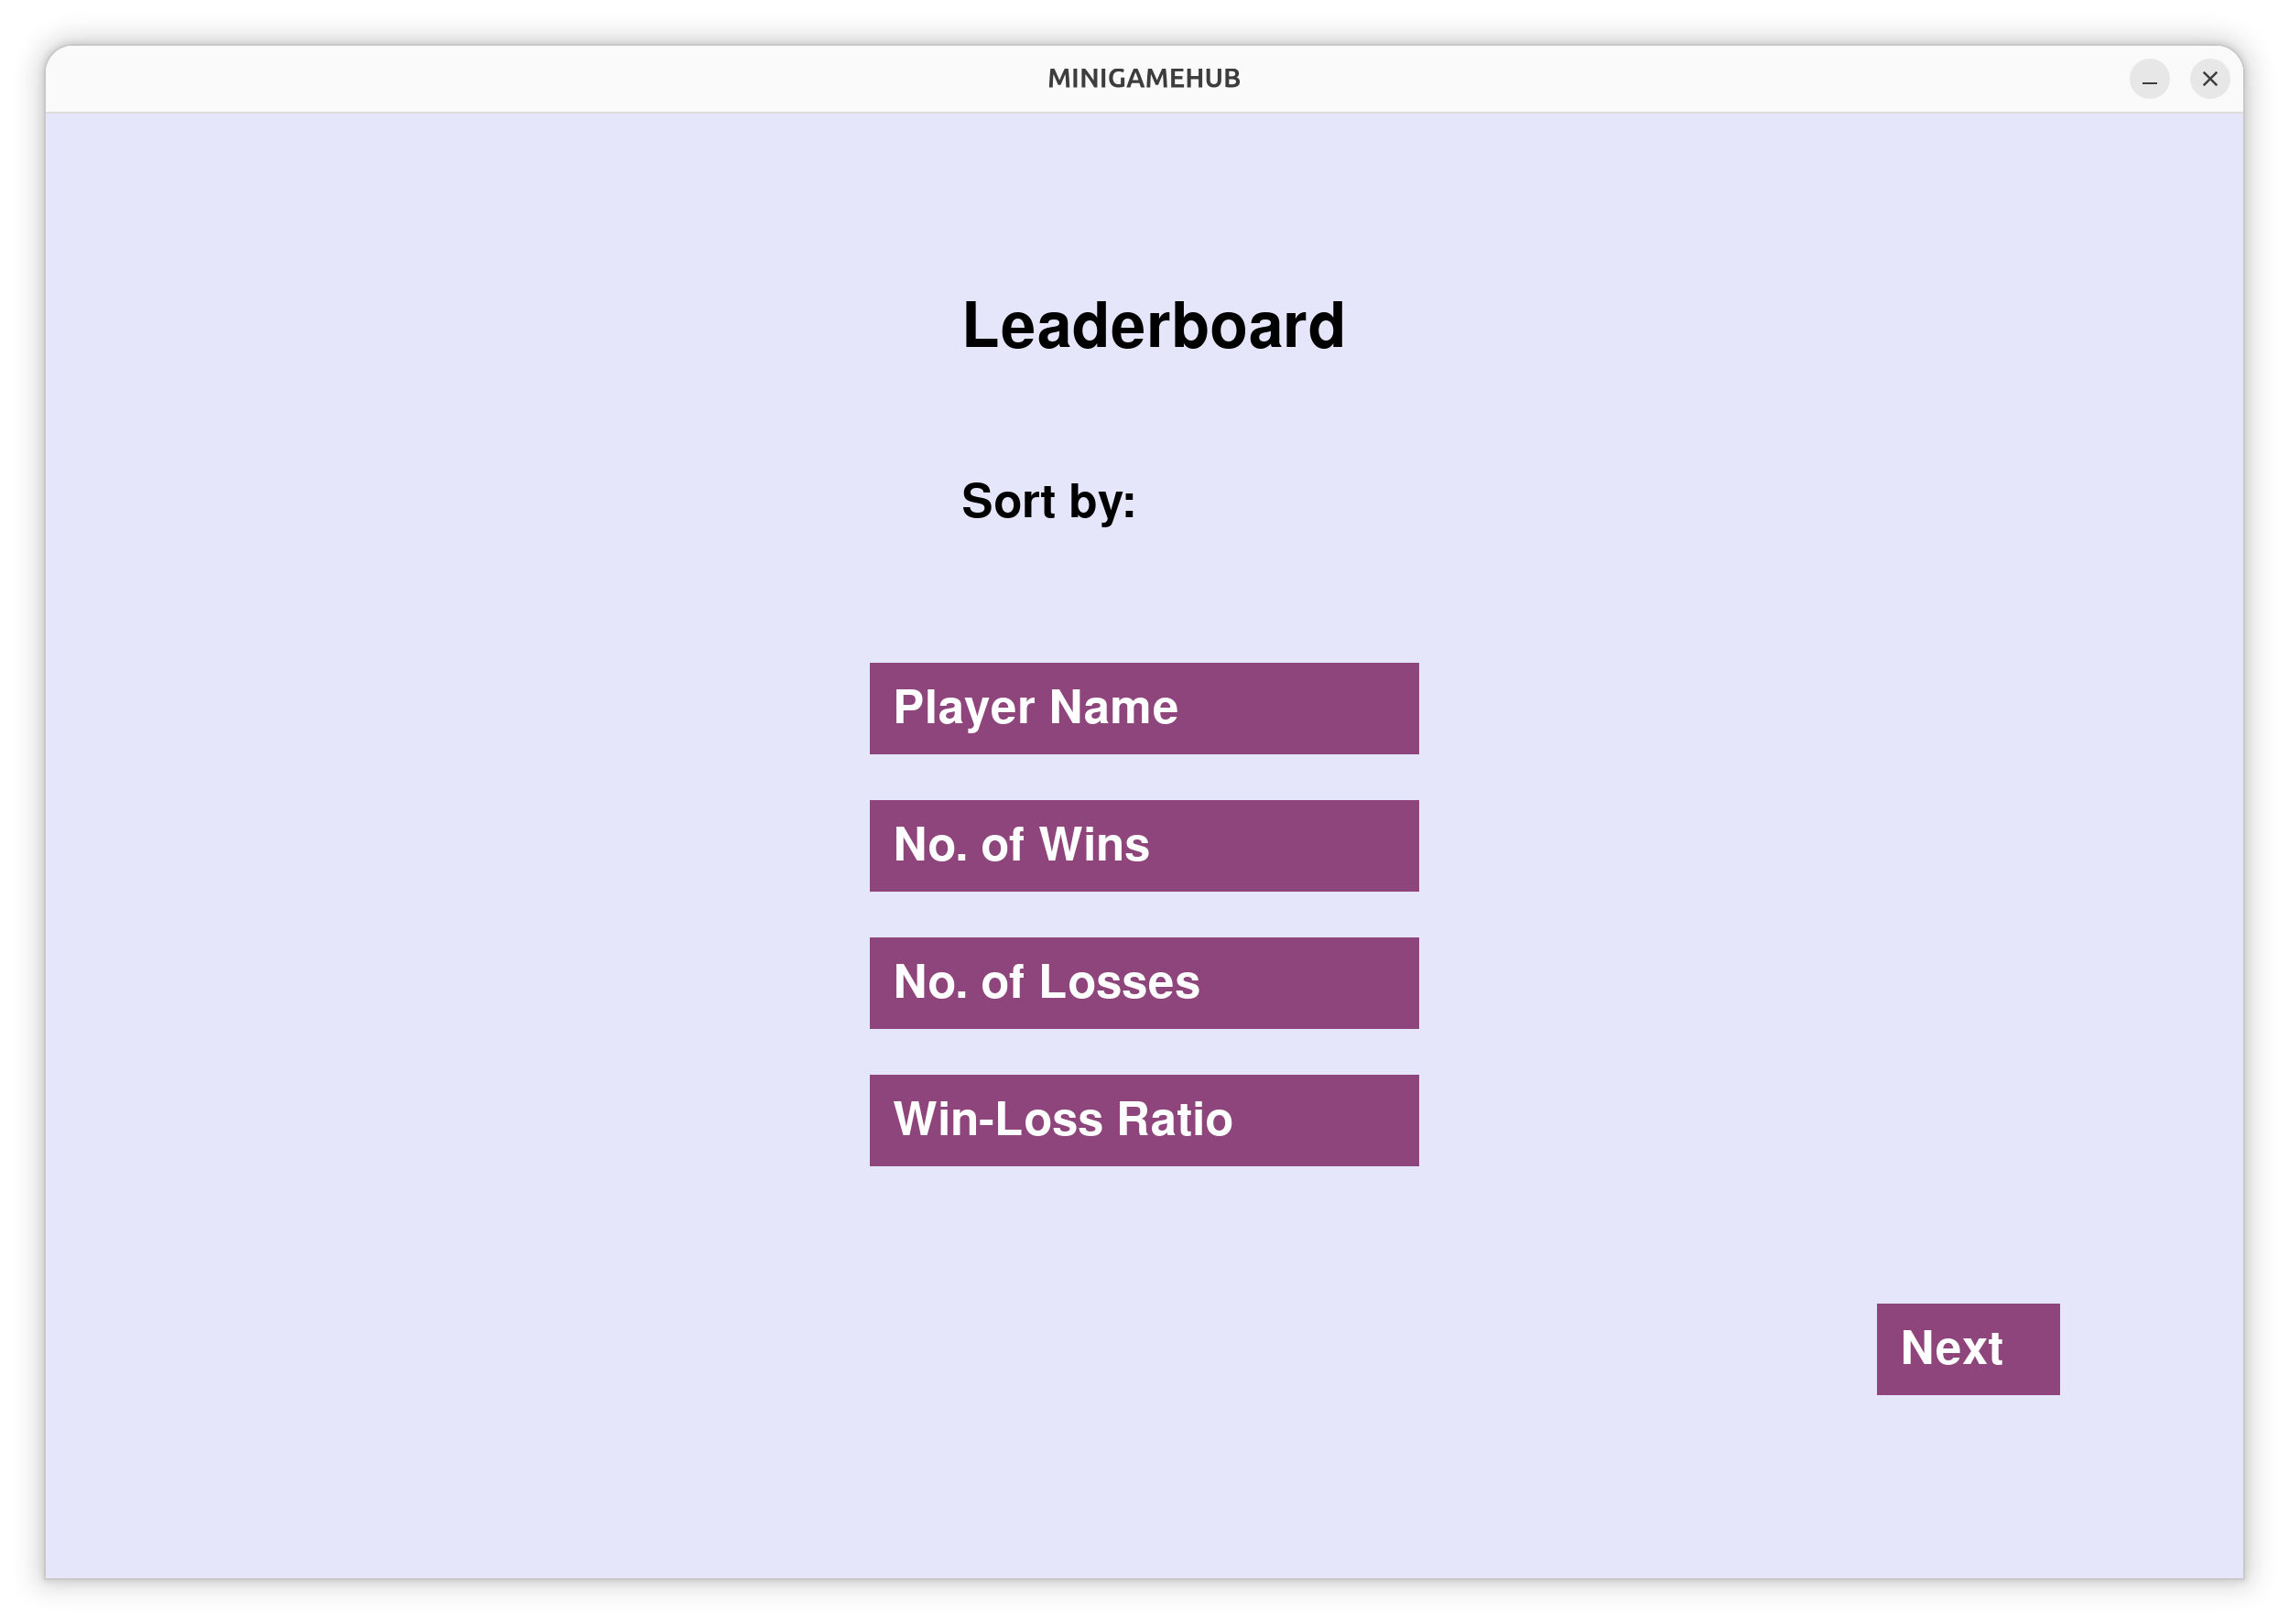
\includegraphics[width=0.7\textwidth]{Images/leaderboard_menu.png}
        \caption{Leaderboard Menu}\label{fig:Leaderboard Menu}
    \end{figure}

 \begin{figure}[h!]
        \centering
        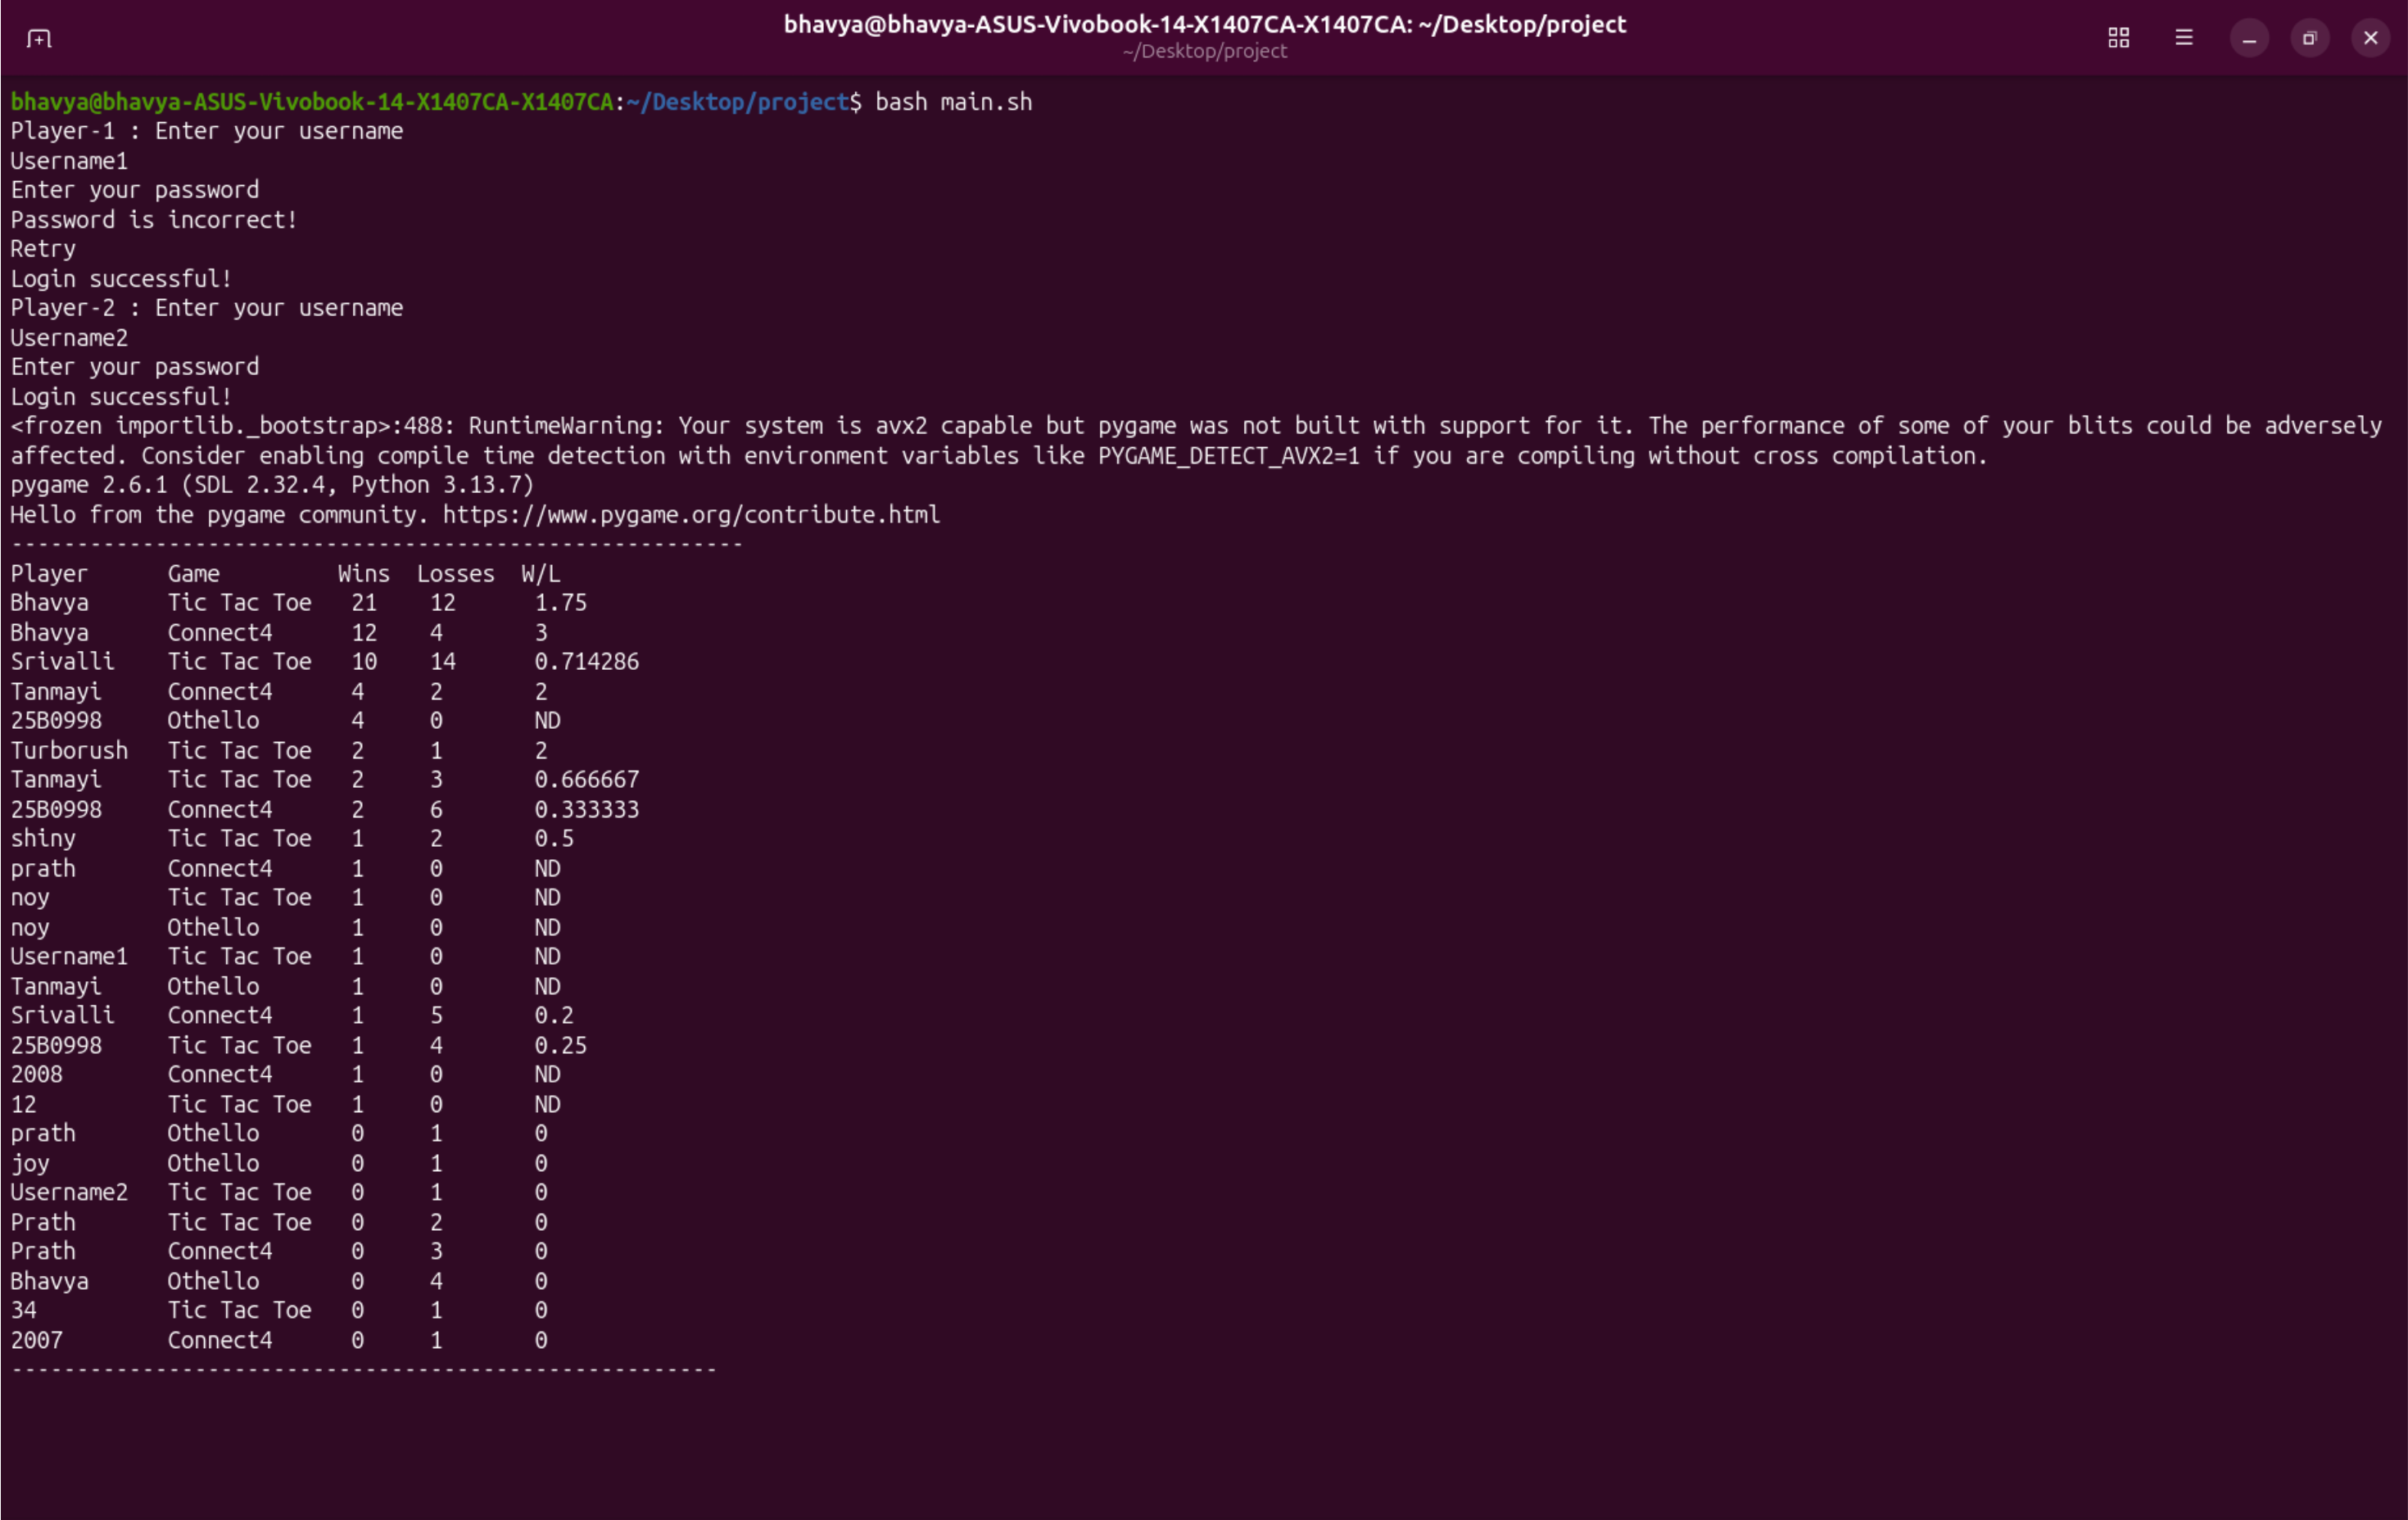
\includegraphics[width=0.7\textwidth]{Images/leaderboard.png}
        \caption{Leaderboard Display}\label{fig:Leaderboard Display}
    \end{figure}

The system also shows simple graphs based on the game data, making it easier to spot things like which games are played the most and which players are doing well. After that, you can choose whether to keep playing or exit the application.
 \begin{figure}[h!]
        \centering
        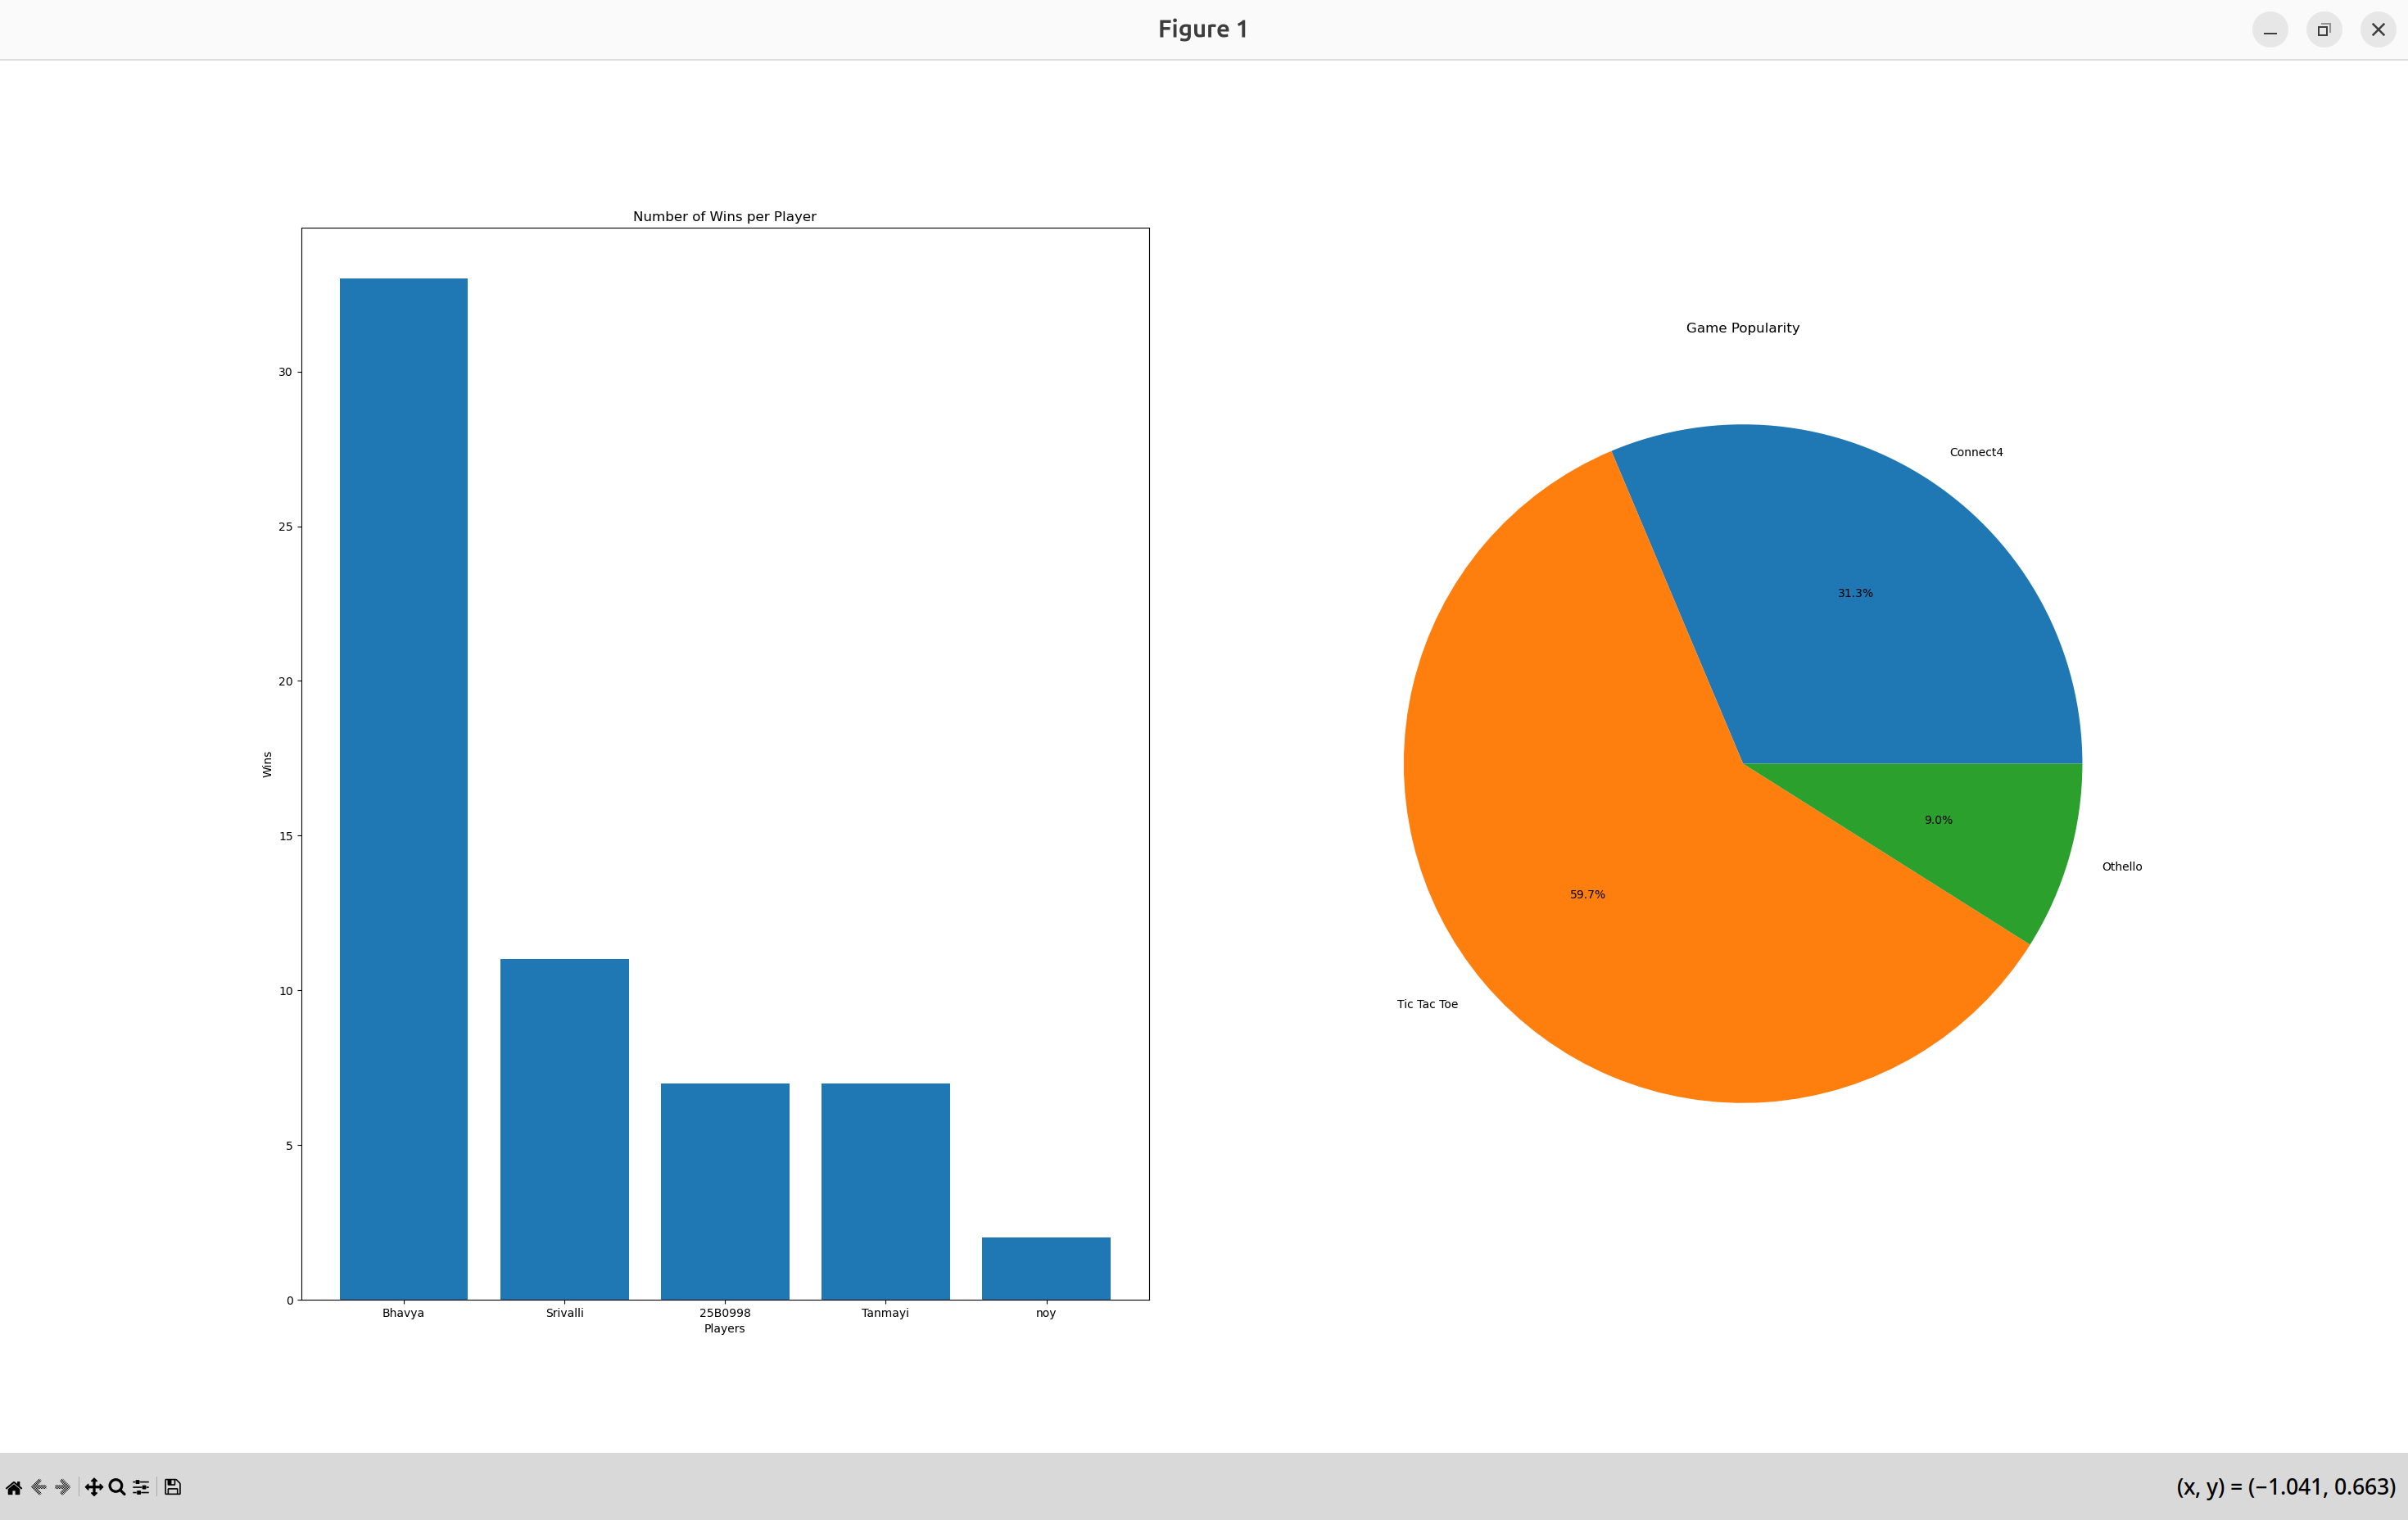
\includegraphics[width=0.7\textwidth]{Images/graph analysis.png}
        \caption{Graphical Analysis}\label{fig:Graphical Analysis}
    \end{figure} 
\subsection{Game Play}
Eachgame in this hub follows a turn based structure, where the players take alternate turns until a win or draw condition is reached.
A basegame class is used to manage the game board, functions like switch turns ,etc. which are common to all the games.
\subsubsection{Tic-Tac-Toe}
Players take turns clicking on the grid to place their X or O wherever they want. After each move, the game quickly checks if someone has formed a winning pattern, and the first player to do so wins the game.
 \begin{figure}[h!]
        \centering
        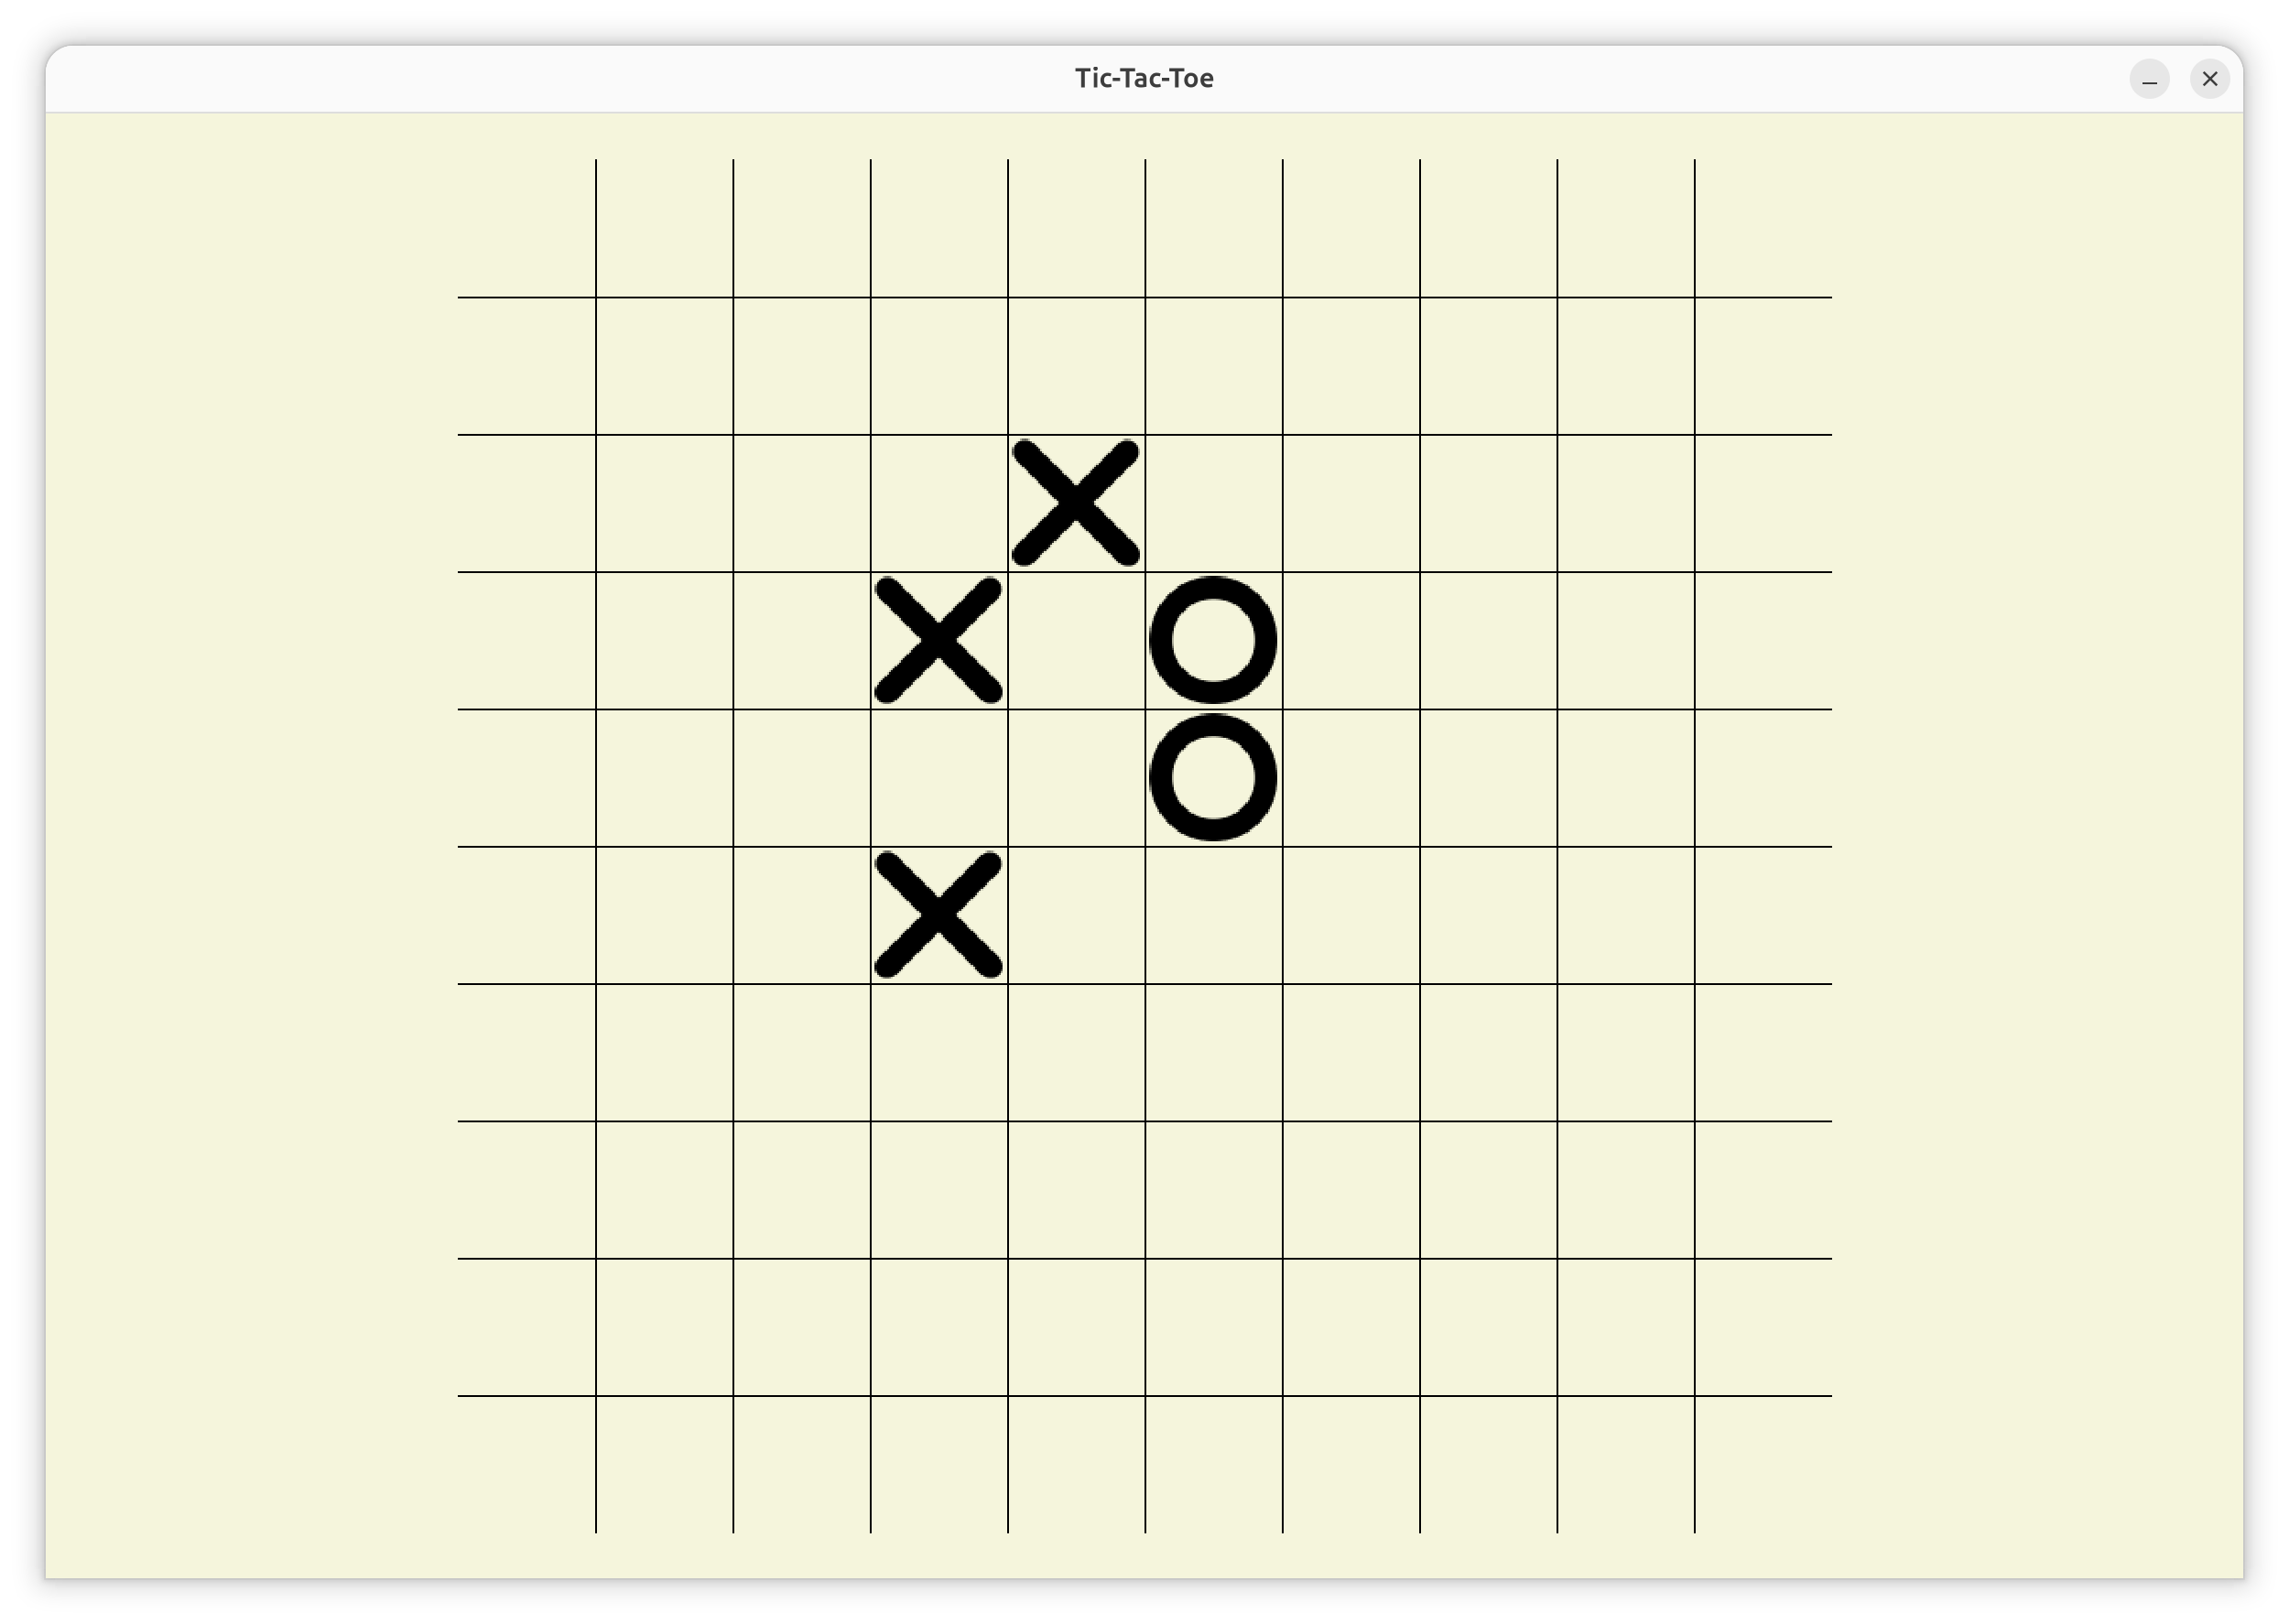
\includegraphics[width=0.7\textwidth]{Images/tictactoe.png}
        \caption{Tic Tac Toe Screen}\label{fig:Tic tac toe Screen}
    \end{figure} 
\subsubsection{Othello}
 Players take turns placing their pieces on the board. You can only make a move if it captures your opponent’s pieces by surrounding them between your new 
 \begin{figure}[h!]
        \centering
        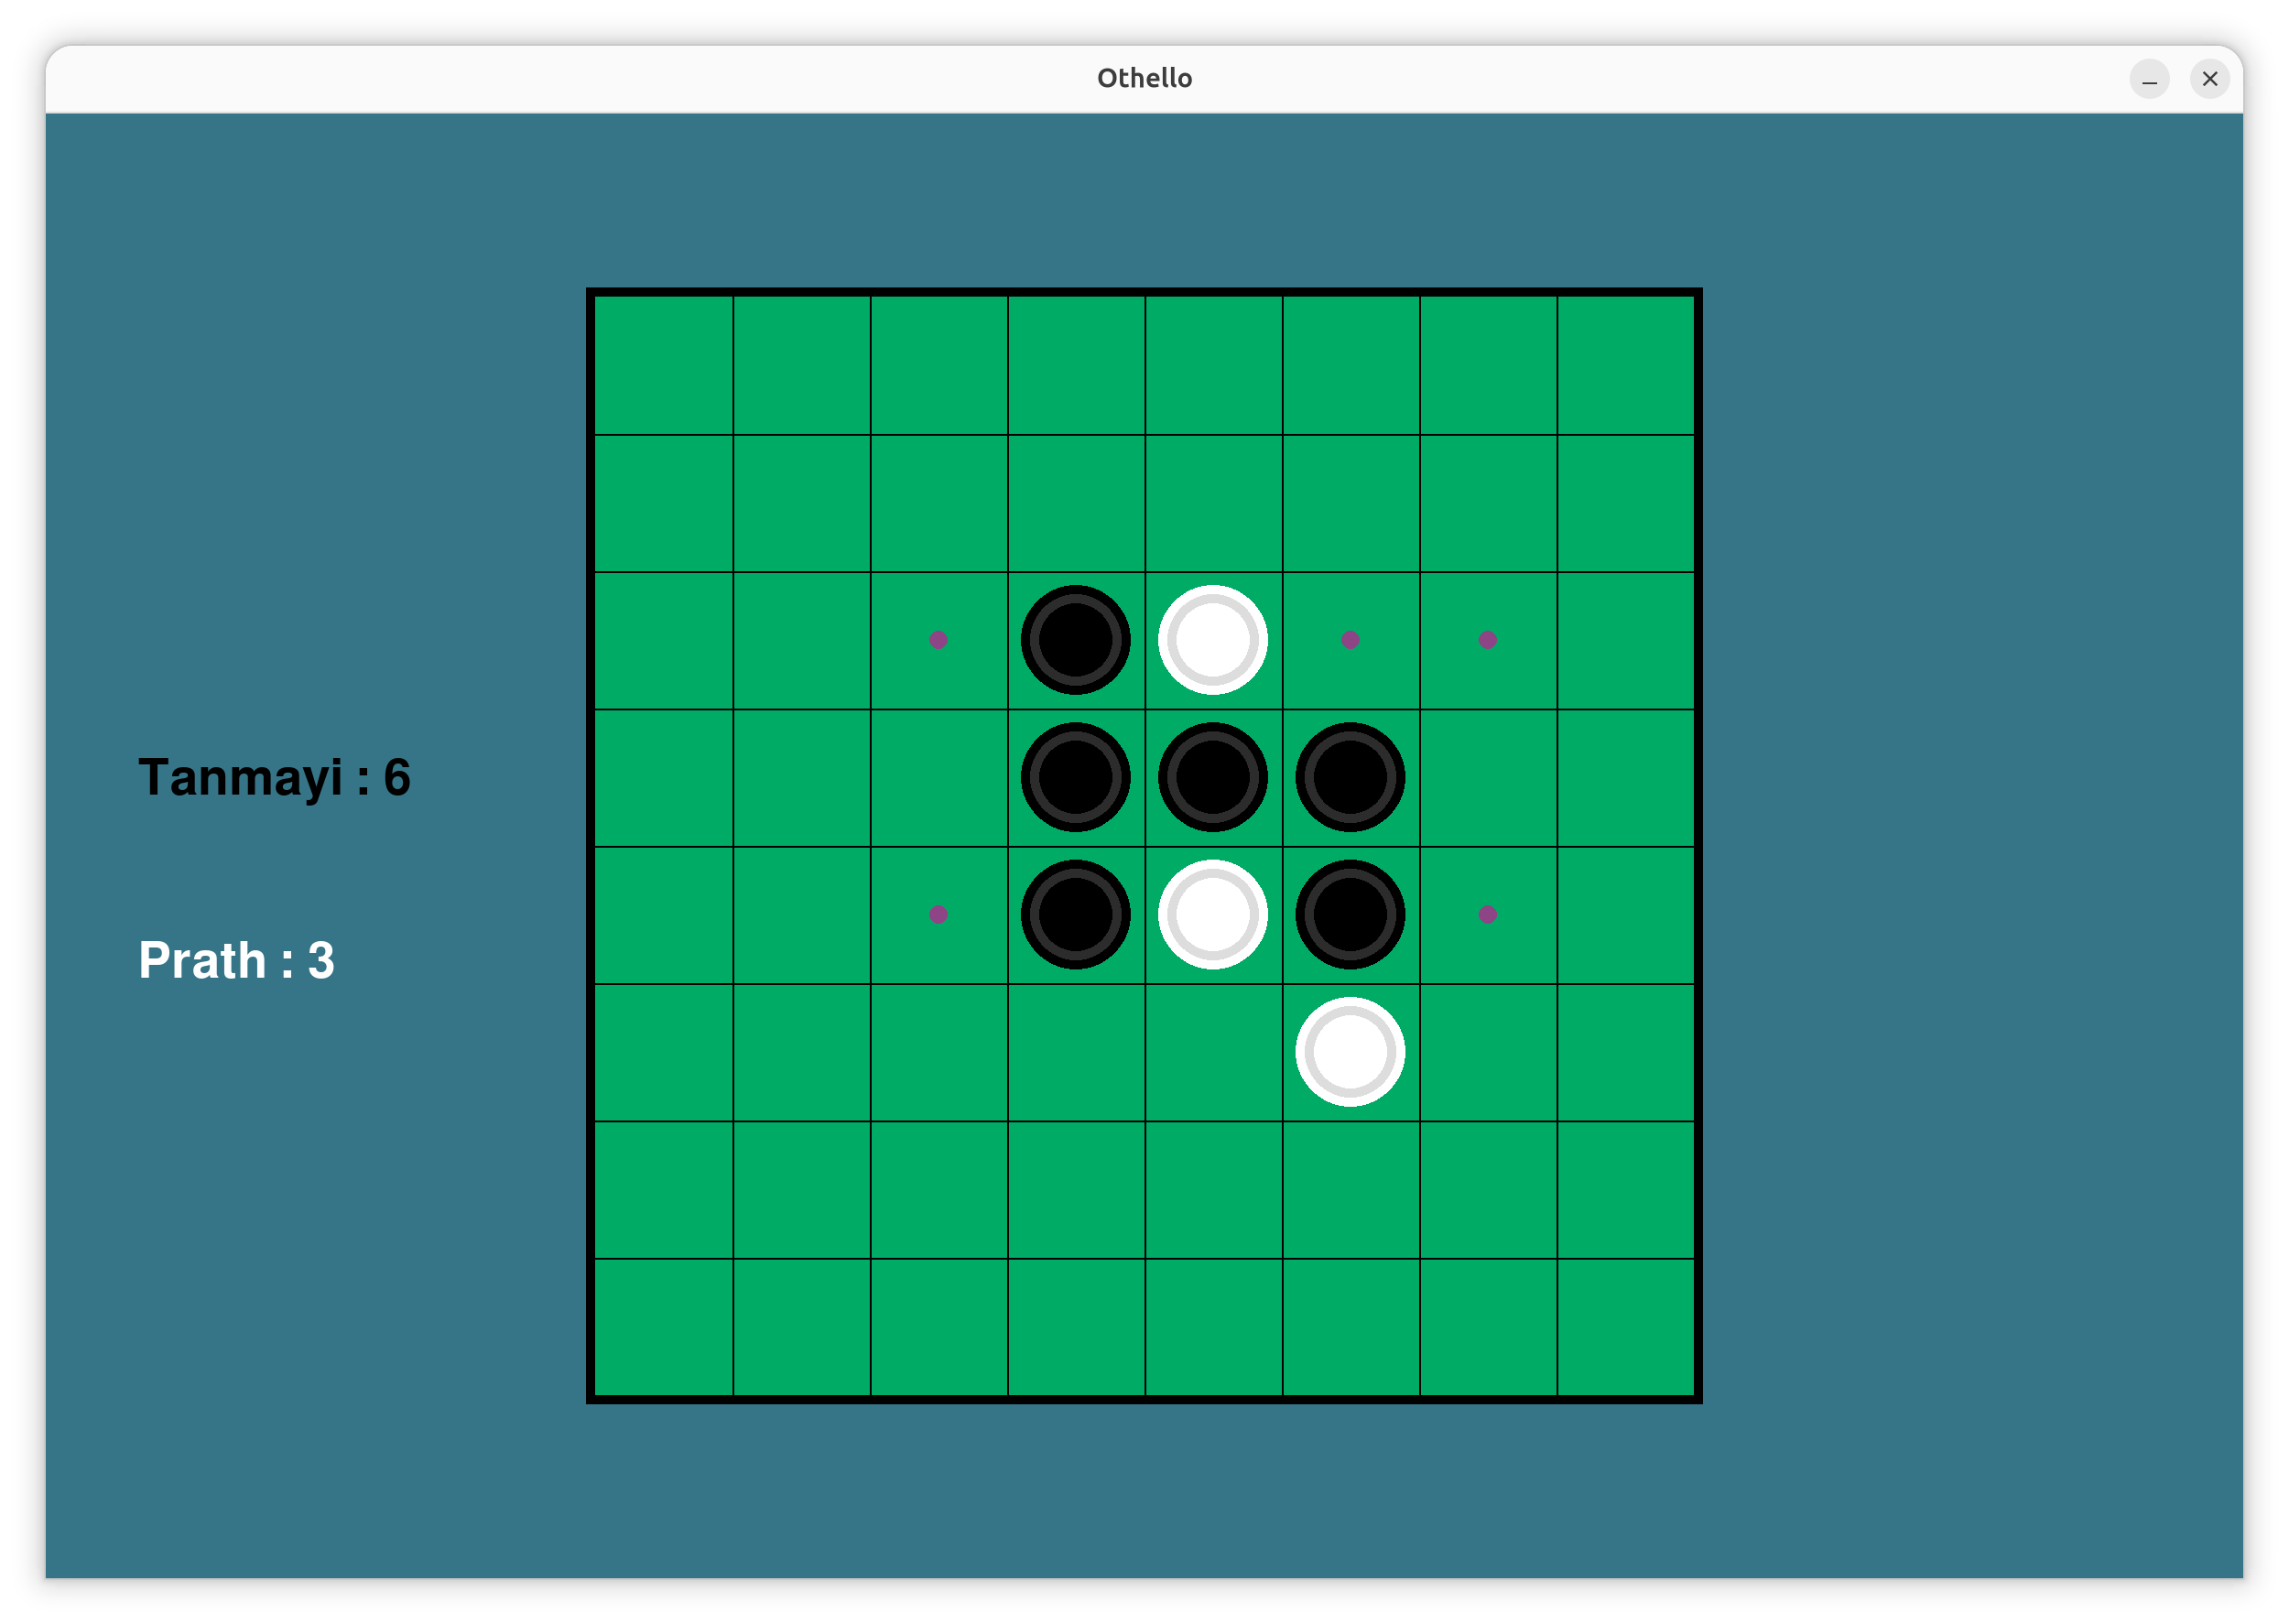
\includegraphics[width=0.7\textwidth]{Images/Othello.png}
        \caption{Othello Screen}\label{fig:Othello Screen}
    \end{figure} 

piece and one of your existing ones—those pieces then flip to your color. The game goes on until neither player has any moves left, and whoever has more pieces on the board at the end wins.

\subsubsection{Connect4}
Players take turns dropping their pieces into any column they choose, and the piece falls to the lowest empty spot. The aim is to connect four of your pieces in a row—either across, up and down, or diagonally. The game also shows a small dropping animation and makes sure the move is valid before placing the piece.
 \begin{figure}[h!]
        \centering
        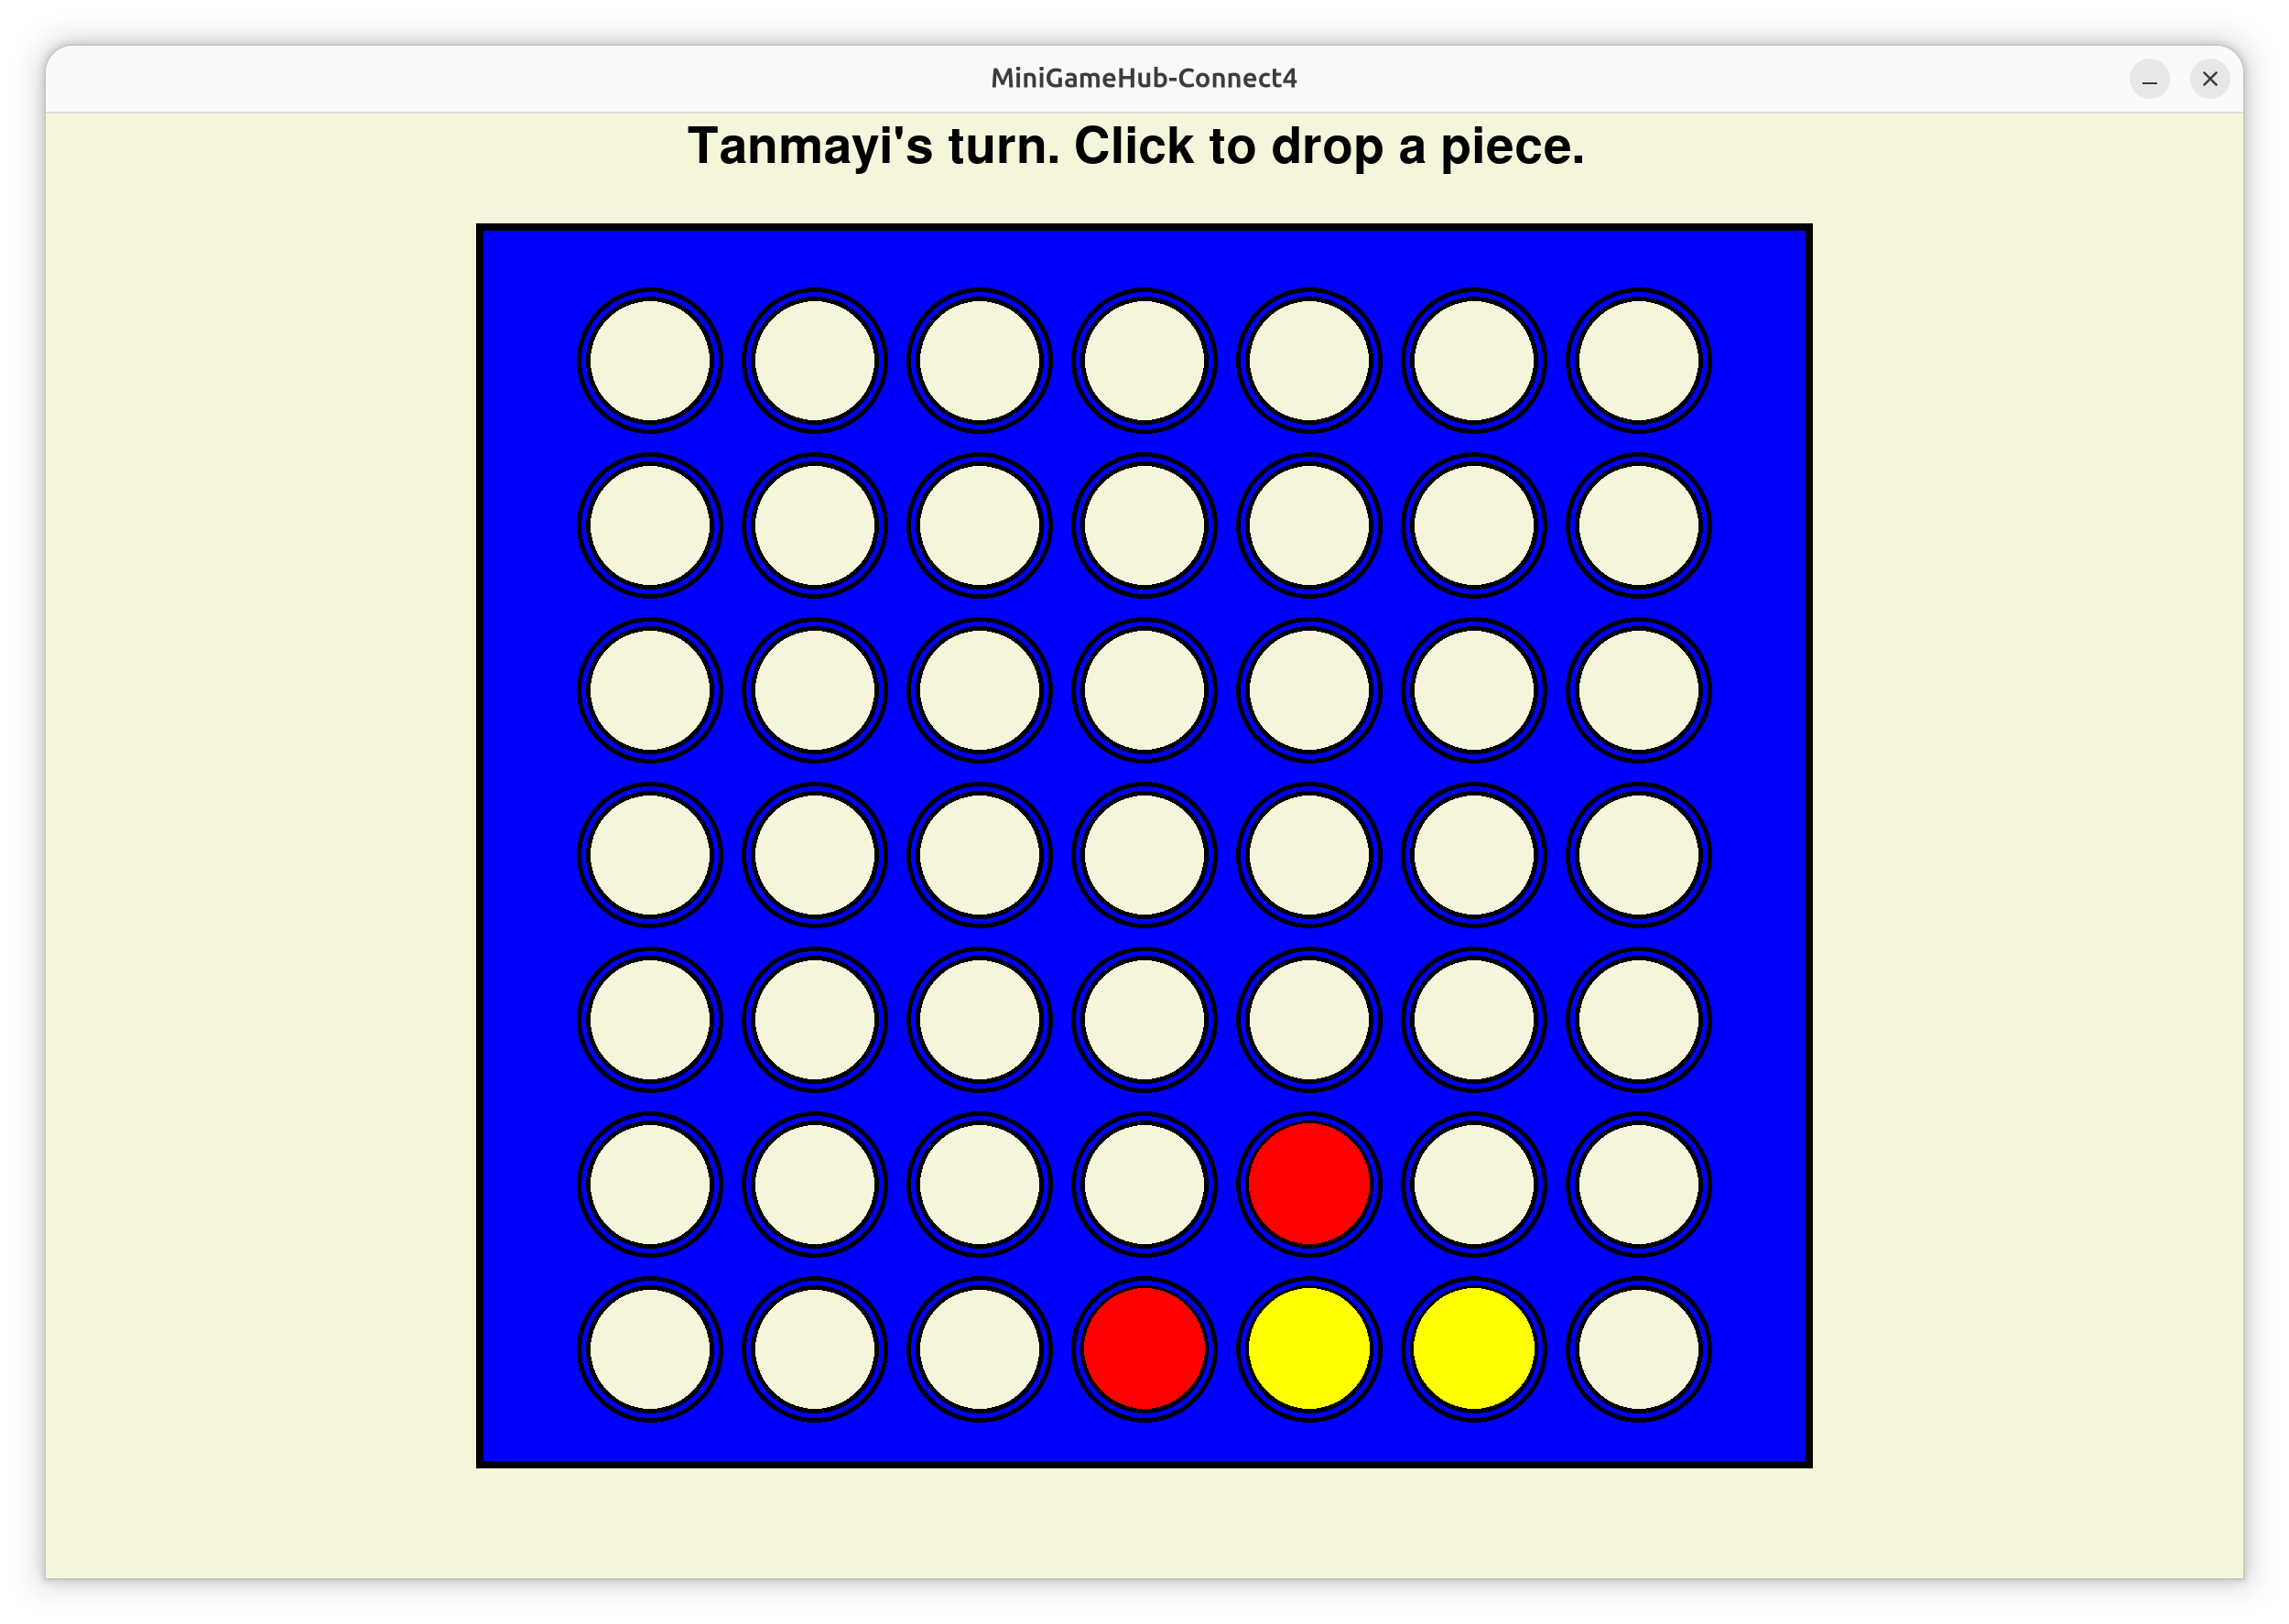
\includegraphics[width=0.7\textwidth]{Images/Connect4.png}
        \caption{Connect4 Screen}\label{fig:Connect4 Screen}
    \end{figure} 

\begin{thebibliography}{9}

\bibitem{pygame}
Pygame-ce Documentation\\
\texttt{https://pyga.me/docs/}

\bibitem{numpy}
NumPy Documentation\\
\texttt{https://numpy.org/doc/}

\bibitem{matplotlib}
Matplotlib Documentation\\
\texttt{https://matplotlib.org/stable/contents.html}

\bibitem{python}
Python Documentation\\
\texttt{https://docs.python.org/3/}

\end{thebibliography}
\end{document}